\section{Filter\hartl{509}}
\subsection{Tiefpass-Filter\hartl{514}}

\subsubsection{1. Ordnung}
\begin{itemize}
  \item Aufbau\\
  \begin{figure}[htb]
  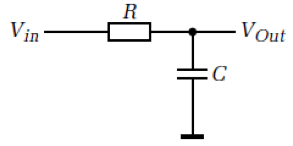
\includegraphics[scale=0.4]{pictures/tiefpass1ordnung}
  \end{figure}
  \item Übertragungsfunktion 
  \begin{equation}
  G1(s)=\frac{1}{1+s\cdot C\cdot R}
  \end{equation}
  \item Zeitkonstante T\\
  Bei $j\omega=\frac{1}{T}$sin Real-  und Imaginärteil gleich gross
  \begin{equation}
  T:=\frac{1}{R\cdot C}
  \end{equation}
  \item $\to$ Amplitude $\frac{1}{1.41}\to 3dB$
  \begin{equation}
  f_{3dB}=\frac{1}{2\pi R\cdot C}
  \end{equation}
  \item Amplitudengang (3dB bei 1kHz)\\
  \begin{figure}[!htbs]
  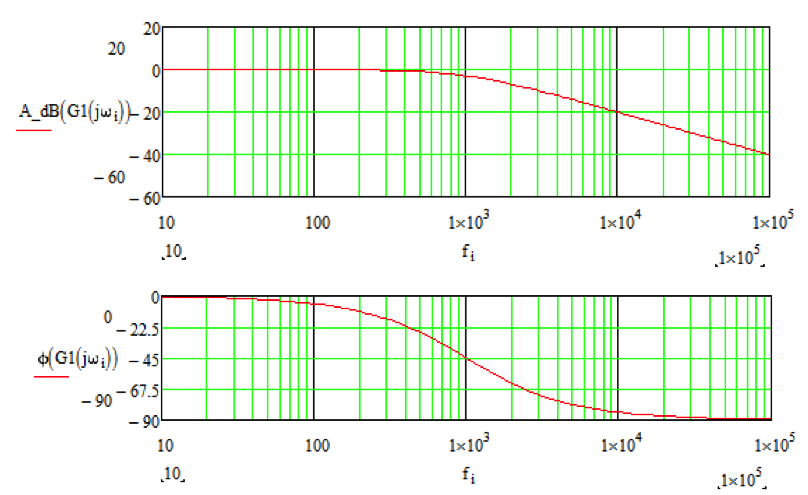
\includegraphics[scale=0.5]{pictures/tiefpass1ordnungamplitude}
  \end{figure}
  
\end{itemize}


\subsubsection{2. Ordnung}
\begin{itemize}
  \item Kaskadierte RC-Tiefpässe\\
  \begin{figure}[htb]
  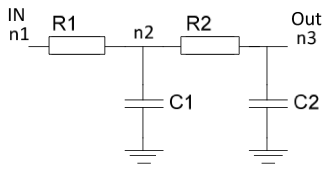
\includegraphics[scale=0.4]{pictures/tiefpass2ordnung}
  \end{figure}
  \item Stromgleichungen für Knoten $n_2$ und $n_3$ (out)
  \begin{gather}
  0=(U_2-U_{in})\cdot \frac{1}{R_1}+(U_2-U_3)\cdot \frac{1}{R_2}+U_2\cdot s\cdot C_1\\
  0=(U_3-U_2)\cdot \frac{1}{R_2}+U_3\cdot s\cdot C_2\\
  U_2=R_2\cdot U_3\cdot (\frac{1}{R_2}+s\cdot C_2)\\
  \text{$U_2$ in oberer Gleichung eingesetzt und aufgelöst für
  $U_{out} /U_{in}$}\notag\\
  G_{p}(s)=\frac{1}{C_1\cdot R_1\cdot s+C_2\cdot R_1\cdot s+C_2\cdot R_2\cdot s+C_1\cdot C_2\cdot R_1\cdot R_2\cdot s^2+1}
  \end{gather}
  Vergleich: Allgemeine Beschreibung von Tiefpass 2. Ordnung mit
  Verstärkung $A_0$, Kreisfrequenz $\omega_{0}$ und Güte Q
  \begin{gather}
  T_{lp}(s)=\frac{A0}{\frac{s^2}{\omega_{0}^2}+\frac{s}{Q\omega_{0}}+1}\\
  A0=1\notag\\
  \omega_{0}=\frac{1}{\sqrt{C_1\cdot C_2\cdot R_1\cdot R_2}}\\
  \text{Güte berechnet mit Termen, die s enthalten}\notag\\
  \frac{s}{Q\cdot \omega_{0}}=C_1\cdot R_1\cdot s+C_2\cdot R_1\cdot s+C_2\cdot R_2\cdot s\\
  Q:=\frac{\sqrt{C_1\cdot C_2\cdot R_1\cdot R_2}}{R_1\cdot (C_1+C_2)+C_2R_2}
  \end{gather}
  Passive RC-Filter können maximal Güte von 0.5 haben (2 identische reelle
  Pole) Filter höherer Güte benötigen Spulen oder Verstärker
\end{itemize}

\subsection{Sallen Key (Einfachmitkopplung)\hartl{517}}
\begin{figure}[htb]
\centering
 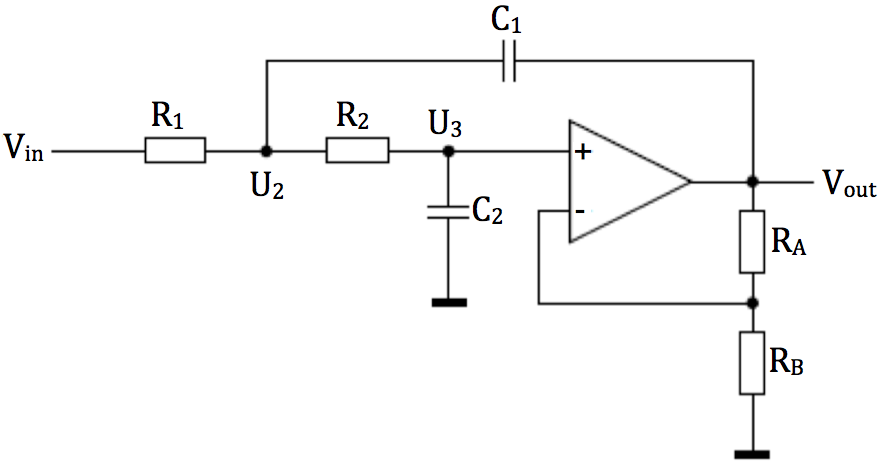
\includegraphics[scale=0.5]{pictures/sallenkey}
\end{figure}
\begin{gather}
0=(U_2-U_{in})\cdot \frac{1}{R_1}+(U_2-U_3)\cdot \frac{1}{R_2}+(U_2-U_{out})\cdot s\cdot C_1\\
0=(U_3-U_2)\cdot \frac{1}{R_2}+U_3\cdot s\cdot C_2\\
\text{Opamp: }U_{out}=G_0\cdot U_3\\
G0=\frac{R_{A}+R_{B}}{R_{B}}\\
G_{SK}(s):=\frac{G0}{C_1\cdot C_2\cdot R_1\cdot R_2\cdot s^2+s\cdot [C_2\cdot
(R_1+R_2)+C_1\cdot R_1\cdot (1-G_0)]+1}\\
\text{Güte:
}Q_{SK}(G_0)=\frac{\sqrt{C_1\cdot C_2\cdot R_1\cdot R_2}}{C_2\cdot (R_1+R_2)+C_1\cdot R_1\cdot (1-G_0)}\\
\text{Grenzfrequenz: }\omega_0=\frac{1}{\sqrt{C_1\cdot C_2\cdot R_1\cdot R_2}}
\end{gather}
\subsubsection{Sallen Key-Filter bei hohen Frequenzen}
\begin{figure}[htb]
\centering
 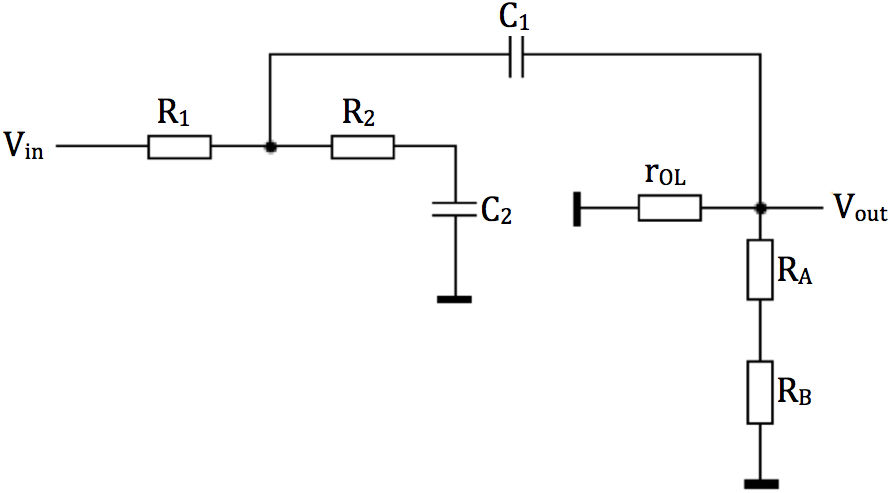
\includegraphics[scale=0.5]{pictures/sallenkey2}
\end{figure}
\begin{itemize}
  \item Wenn der Opamp nicht mehr verstärkt
  \item $C_1$, $C_2$ wirken wie Kurzschlüsse
  \begin{equation}
  \frac{V_{Out}}{V_{in}}=\frac{r_{OL}\parallel R_2\parallel
  (R_{A}+R_{B})}{R_1+r_{OL}\parallel R_2\parallel (R_{A}+R_{B})}\approx
  \frac{r_{OL}}{R_1+r_{OL}}
  \end{equation}
  \item Folge: Sallen Key-Filter sind nicht geeignet für Systeme mit hohen
  Frequenzanteilen, z.B. PEM-DAC
\end{itemize}


\subsection{Multiple Feedback\hartl{522}}
\begin{figure}[!h]
\centering
 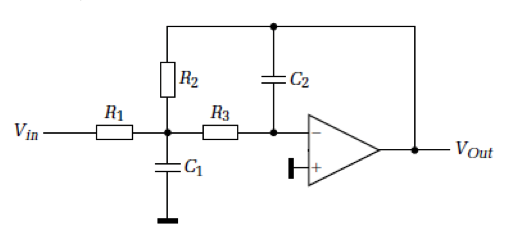
\includegraphics[scale=0.5]{pictures/mulipleFeedback}
\end{figure}
\begin{gather}
0=(U_2-U_{in})\cdot \frac{1}{R_1}+(U_2-U_{out})\cdot \frac{1}{R_2}+(U_2-U_3)\cdot \frac{1}{R_3}+U_2\cdot s\cdot C_1\\
0=(U_3-U_2)\cdot \frac{1}{R_3}+(U_3-U_{out})\cdot s\cdot C_2\\
\text{Opamp sorg für }U_3=0\notag\\
G_{mf}(s)=\frac{G0}{1+C_2(R_2+R_3+R_3\cdot \frac{R_2}{R_1})\cdot s+C_1\cdot C_2\cdot R_2\cdot R_3\cdot s^s}\\
Q_{mf}=\frac{\sqrt{C_1\cdot C_2\cdot R_2\cdot R_3}}{C_2\cdot (R_2+R_3+R_3\cdot \frac{R_2}{R_1})}
\end{gather}
Die Güte wird v.a. eingestellt mit $C_2$ und $R_1$, grosse Güte für kleines
$C_2$ und grosses $R_1$. $C_2$ beeinflusst auch das Frequenzverhalten, $R_1$ die
Verstärkung.

\subsection{Zustandsvariablen-Filter}
\begin{figure}[!h]
\centering
 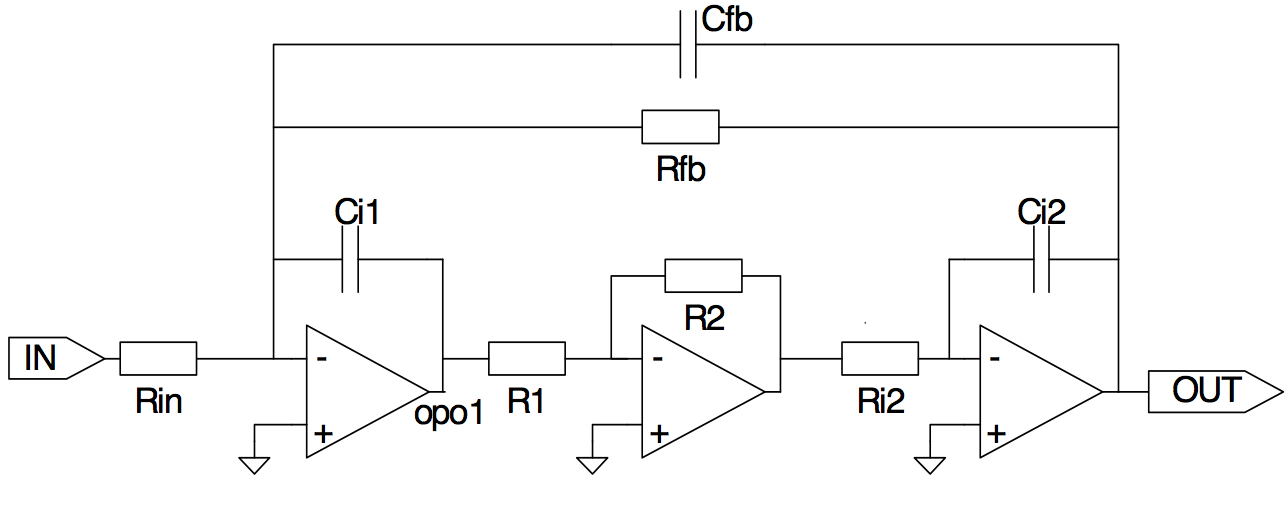
\includegraphics[scale=0.5]{pictures/zustandsvariable}
\end{figure}
\begin{gather}
V{out}=-\frac{1}{s\cdot C_{i2}\cdot R_{i1}}\cdot V_{opo2}\\
V_{opo2}=-\frac{R_2}{R_1}\cdot V_{opo1}\\
V_{opo1}=\frac{-1}{s\cdot C_{i1}}\cdot (\frac{V_{in}}{R_{in}}+\frac{V_{out}}{R_{fb}}+s\cdot C_{fb}\cdot V_{out})\\
G_{ss}(s)=\frac{-\frac{R_{fb}}{rin}}{C_{i1}\cdot C_{i2}\cdot R_{i1}\cdot R_{fb}\cdot \frac{R_1}{R_2}\cdot s^2+C_{fb}\cdot R_{fb}\cdot s+1}\\
\omega_{0}=\frac{1}{\sqrt{C_{i1}\cdot C_{i2}\cdot R_{i1}\cdot R_{fb}\cdot \frac{R_1}{R_2}}}\\
A0=-\frac{R_{fb}}{Rin}\\
Q=\frac{\sqrt{C_{i1}\cdot C_{i2}\cdot R_{i1}\cdot R_{fb}\cdot \frac{R_1}{R_2}}}{C_{fb}\cdot R_{fb}}
\end{gather}
D.h. mit dieser Topologie sind alle 3 Parameter frei wählbar!
\begin{enumerate}
  \item $\omega_{0}$ mit $C_{i1}$, $C_{i2}$, $R_{fb}$, $R_{i2}$, $R_1$, $R_2$
  \item Q mit $C_{fb}$
  \item $A_0$ mit $R_{in}$
\end{enumerate}


